\section{Data and experimental design}
\label{sec:design}
\paragraph{Frozen public matrices.}
HELM MMLU~\citep{hendrycks2021mmlu,liang2023helm} release v1.13.0 (dated 2025-01-10) supplies exact-match scores for 79 models on all 57 MMLU subjects. All rows are complete; no model is removed for missing scores. The source's evaluation counts range from 100 to 1,534 across reported cells. Equal subject weighting therefore differs from pooling all test examples and is a study design, not an assertion that we reproduce HELM's displayed aggregate weighting. Open LLM Leaderboard contents~\citep{openllmcontents2025} at commit \texttt{9c09a7cae43334062a82cb164f2ef255013dafa2} supplies 4,576 evaluations on IFEval, BBH, MATH Level 5, GPQA, MUSR and MMLU-PRO. We exclude one source-flagged evaluation and retain 4,575 complete rows. Primary scores are the six published normalized columns divided by 100; we verify their mean exactly reproduces the published average. These matrices are analyzed separately: a subject and a broad task are different units of investment.

Open LLM rows identify model--precision evaluations, so related models and repeated model names are not independent experimental draws. We retain the public evaluation population for the primary comparison and use a deterministic one-row-per-model-name sensitivity with 4,496 entries. A separate sensitivity uses the six raw score columns in their supplied $[0,1]$ units. HELM has no zero cells; the primary Open LLM matrix has 384. We preserve zeros rather than adding offsets to geometric means. Acquisition on 2026-11-03 records all URLs, byte counts and SHA-256 hashes in \texttt{data/manifest.json}; preparation and exclusion counts are in \texttt{data/processed/audit.json}.

\paragraph{Cohorts and outcomes.}
We compute budgets for every retained target, all five rules and all five gain/ceiling settings. For primary paired comparisons we remove the \emph{union} of incumbent winners across rules, leaving 77 HELM and 4,571 Open LLM common challengers. This avoids comparing a zero-cost incumbent for one rule with a genuine challenger for another. We also report the full cohorts, with incumbents included. Bounded-gain reachability uses those fixed full cohorts; conditioning budgets on rule-specific reachable subsets would confound the comparison with a change in targets. We report budget distributions, paired counts and the fraction reachable within each budget. Infeasible targets stay in the denominator.

\paragraph{Random task selection.}
A baseline selects tasks in a uniformly random order and applies the same intervention until co-first. On six tasks, success at each budget is the exact fraction of subsets of that size which succeed. The expected first-success count follows from the survival probabilities. For HELM we use 256 independent random task permutations per reachable target and setting, seed 20261103. If no subset can succeed, a stopping code of $n+1$ denotes censoring, not an achievable investment. Full-cohort censored stopping means assign that known value to every provably infeasible target; success probability at a target's own optimal budget is defined only when that budget is finite and is labelled reachable-only with its denominator. Main full-gain comparisons have no infeasible targets. Wilson intervals describe per-target Monte Carlo success probabilities; conservative Hoeffding intervals describe cohort-mean stopping counts. Neither estimates uncertainty in the published model scores.

\paragraph{Sensitivity and verification.}
We repeat the full intervention grid for strict first place; analyze raw scores and unique model names at the primary setting; resample 57 HELM task columns with replacement in 200 seeded designs; and delete each of the six Open LLM tasks in turn. These perturbations assess dependence on benchmark composition. They are not confidence intervals for latent model quality. Scores are fixed published aggregates without repeated runs sufficient to estimate evaluation noise. All 278,055 attack records finish with exact/optimal or infeasible status and zero unresolved optima. We additionally check monotonicity, independently recompute 400 reported winners including full Borda reranking, and compare optimizers against exhaustive enumeration in 120 small validation cases with ties and zeros (seed 47). These validation cases check algorithms and are excluded from empirical claims.

\section{Results}
\label{sec:results}
\subsection{Full improvements separate Borda from cardinal rules}
Table~\ref{tab:primary} and Figure~\ref{fig:budget} report the common-challenger comparison. Under full unit-ceiling improvement, every target can reach co-first for every rule. On common challengers, median budgets for mean, median, geometric mean, minimum and Borda are respectively 16, 21, 16, 12 and 48 of 57 HELM subjects; Open LLM medians are 2, 3, 3, 3 and 6 of 6 tasks. These are finite-cohort descriptions of optimal task counts. They are neither estimates of training resources nor comparisons of equal effort between benchmarks.

\begin{table}[t]
\caption{\PrimaryBudgetsCaption}
\label{tab:primary}
\centering
\input{tables/primary_budgets}
\end{table}
\begin{figure}[t]
\centering
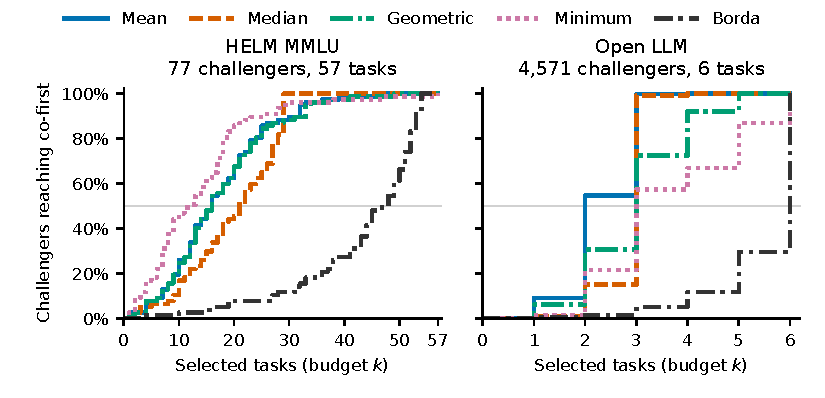
\includegraphics[width=\linewidth]{figures/budget_curves.pdf}
\caption{\BudgetCurvesCaption}
\label{fig:budget}
\end{figure}

The paired comparison (Appendix Table~\ref{tab:paired}) is stronger than a comparison of medians alone. Every HELM common challenger needs more selections under Borda than mean. For Open LLM, Borda costs more for 4,544 challengers and ties for 27; none is cheaper. The same zero-cheaper result holds against geometric mean in these primary cohorts. Yet this is not a universal ordering of the five rules: Borda is cheaper than minimum for one HELM challenger and 16 Open LLM challengers, and cheaper than median for 16 Open LLM challengers. Mean is cheaper than median for 64 HELM challengers, ties for two, and costs more for 11. The full per-target records and paired counts allow these exceptions to be checked.

Including incumbents changes the HELM Borda median from 48 to 46 and minimum from 12 to 11; other HELM medians and all Open LLM medians above are unchanged. The lone full-cohort Open LLM case in which Borda is cheaper than mean is Borda's existing winner, whose budgets are zero and one. Removing the common incumbent union prevents this special case from being mistaken for a challenger advantage.

The mechanism is consistent with the exact formulations. Mean improvements can concentrate on large score gaps; median success depends on crossing a threshold in enough coordinates; minimum success depends on repairing every coordinate below a possibly low rival minimum. Borda converts each task improvement into rank crossings against all rivals. Reaching the cardinal ceiling can therefore buy many cardinal-score units without buying sufficient rank points to overtake a broad-task leader. The empirical separation arises from these observed profiles and opponents, rather than from a theorem that Borda always requires more tasks.

\subsection{Restricting gains changes who can reach first}
Figure~\ref{fig:gain} shows fixed-cohort reachability. At quarter-headroom improvement ($\alpha=0.25$, unit ceilings), reachable HELM counts for mean, median, geometric mean, minimum and Borda are 9, 11, 9, 21 and 10 out of 79. Open LLM counts are 558, 427, 841, 4,575 and 480 out of 4,575. The minimum remains reachable for every Open LLM target while most targets are infeasible under the other rules. Its first-place threshold is the largest rival's weakest score; it need not require uniformly high scores. Thus a rule that penalizes weak tasks can still permit inexpensive selective improvements relative to its own leader.

\begin{figure}[t]
\centering
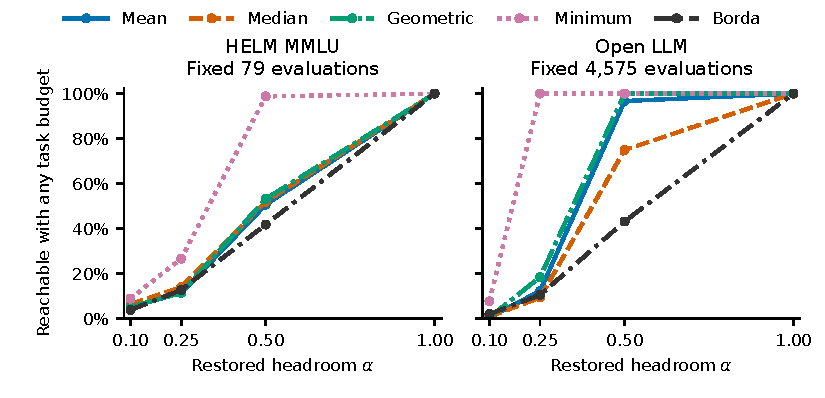
\includegraphics[width=\linewidth]{figures/gain_reachability.pdf}
\caption{\GainReachabilityCaption}
\label{fig:gain}
\end{figure}

The fixed-cohort reachability curves show this change without silently removing hard targets. Smaller medians among reachable targets would not demonstrate increased robustness or vulnerability: a tighter gain constraint changes the reachable cohort. The observed-maximum ceiling offers a second intervention restriction using scores already achieved in the snapshot; its full results are included with the same fixed denominators. On the common challengers, replacing unit ceilings with observed maxima raises mean's median from 16 to 37 on HELM and from 2 to 4 on Open LLM, while Borda changes from 48 to 49 and remains 6, respectively (Appendix Table~\ref{tab:ceiling}). All measured budgets and reachability patterns satisfy the expected monotonicity in gain and ceiling.

\subsection{Targeting and random selection are different resources}
Appendix Table~\ref{tab:random} reports all five rules. On full-gain HELM, the minimum rule's mean optimal count is 13.19 tasks, while random task ordering requires an estimated 50.46 on average, with a conservative 95\% Monte Carlo interval of $[49.91,51.02]$. For the mean rule the corresponding counts are 16.70 and 27.24 ($[26.69,27.79]$ for the random mean). Borda's mean counts are 42.23 and 47.89 ($[47.34,48.44]$). Random-order intervals are conditional on the published matrix and concern only permutation sampling. The optimized counts are exact descriptions of that matrix.

These comparisons show that a low minimum budget does not mean arbitrary task selection is effective. In particular, minimum aggregation requires repairing specific weak coordinates, whereas random ordering may encounter the last necessary repair near the end. On Open LLM, the six-task random baseline is enumerated exactly; it has no Monte Carlo error. The accompanying outputs record both stopping counts and success probability at each target's optimized budget.

\subsection{What survives sensitivity checks}
Appendix Table~\ref{tab:robustness} and Figure~\ref{fig:composition} summarize sensitivity. The one-row-per-model Open LLM cohort retains the primary medians 2, 3, 3, 3 and 6. Raw scores retain mean/median/geometric/Borda medians of 2/3/3/6, but change minimum's median from 3 to 5. The raw representation also contains a common challenger where Borda is cheaper than mean, so the primary zero-exception comparison must remain explicitly conditional on the published normalized matrix. Changing normalization changes both score gains and, for cardinal rules, the identity and threshold of the strongest rival.

Across 200 HELM task-resampling designs, the mean rule's cohort median budget ranges from 14 to 19 and Borda's from 43 to 49. The central 95\% empirical design ranges are 14--18 and 45--48. Minimum varies more widely, from 6 to 25 (central range 8--22). Across all six Open LLM task deletions, mean's median is always 2 and Borda's always 5 out of the remaining five tasks; minimum ranges from 2 to 4. The paired median mean-minus-Borda budget difference stays negative in every composition design. These are composition sensitivities on fixed evaluation cohorts; exchangeable task resampling does not capture correlated subjects or test-example sampling noise.

Strict-first sensitivity changes some budgets but preserves the broad primary separation. Across the complete gain/ceiling grid, HELM has 6 changed Borda, 28 changed median and 12 changed minimum budgets among jointly reachable cases, with no target-setting case reachable only under co-first. Open LLM has 6 changed Borda budgets among jointly reachable cases and one Borda case reachable only under co-first. These counts span the full grid, rather than just the primary intervention. Exact zero-margin ties should therefore be reported explicitly, especially when imposing observed ceilings.
